\documentclass[12pt,a4paper]{article}

% incluyendo paquetes
\usepackage[utf8]{inputenc}
\usepackage[spanish]{babel}
\usepackage{milibreria}

\graphicspath{{C:/Users/HUAWEI/Pictures/imagesppt/}} %\incluye todos las imágenes de esa ruta
%\graphicspath{{D:/proyectos_latex/7mo_semestre/gestion_redes/informe_de_redes/main/images}}
\begin{document} % inicio  de documento 



\begin{titlepage}
    %\begin{tikzpicture}[overlay, remember picture]
    %    \fill[red] (10cm,-10cm) rectangle (5cm,-15cm);
    %\end{tikzpicture}
    
    \miRectangulo{-2cm}{-4cm}{2cm}{5cm}{rosado}
%   \miRectangulo{x     }{y }{x1    }{y1   }{color}
    
    \miRectangulo{-1.5cm}{-2cm}{-1.2cm}{23.5cm}{black} % 1
    \miRectangulo{-1.8cm}{23.5cm}{5.7cm}{23.2cm}{black} % 2
    \miRectangulo{5.025cm}{23.5cm}{5.33cm}{20cm}{black} % 3
    \miRectangulo{-2.7cm}{-1.7cm}{4.7cm}{-2cm}{black} % 4
    \miRectangulo{4.2cm}{-2cm}{4.5cm}{10cm}{black} % 5

    \begin{textblock}{100}(100,20)
        \begin{flushright}
        {\huge{\textbf{Universidad Nacional del Altiplano}}}\\
        {\normalsize{\textbf{Educando mentes, Cambiando el mundo}}}
        \end{flushright}
        
    \end{textblock}
    
    \begin{tikzpicture}[remember picture, overlay]
        \node at (current page.north west) [anchor=north west, xshift=120mm, yshift=-47mm] {\includegraphics[width=0.45\textwidth]{\logoright}};
    \end{tikzpicture}
    \begin{textblock}{100}(100,130)
        \begin{flushright}
            {\Large{\textbf{Facultad de Ingeniería Mecánica Eléctrica,
                    Electrónica y Sistemas}}}\\[10pt]
            {\large{\textbf{Escuela Profesional de Ingeniería\\ de Sistemas}}}
        \end{flushright}
    \end{textblock}

    \begin{textblock}{200}(10,163)
        \begin{center}
            
            %\textcolor{azul}{\rule{\linewidth}{0.80mm}}
            % titulo del articulo
            {\LARGE {\textbf{ Tipos de Auditoria }}} \par

            \textcolor{azul}{\rule{0.5\linewidth}{0.80mm}} \par
            \vspace{8mm}
            {\large{\textbf{ Auditoría en sistemas }}} \\[10pt]
            {\large{\textbf{\textcolor{azul}{ing. TICONA YANQUI FIDEL ERNESTO }}}} \\[20pt]
            {\large{\textbf{estudiante}}}\\[10pt]
            {\large{\textbf{$\looparrowright$   Larota Pilco David Brahyan  $\looparrowleft$ }}}\\[5pt]
            %{\large{\textbf{$\looparrowright$    Quispe Calcina Royer $\looparrowleft$ }}}\\[5pt]
            %{\large{\textbf{$\looparrowright$    Rojas Alejo Bruno $\looparrowleft$ }}}\\[5pt]
            %{\large{\textbf{$\looparrowright$  $\mathfrak{David\ Brahyan\ Larota\ Pilco}$   $\looparrowleft$ }}}\\[20pt]
            \today

        \end{center}
    \end{textblock}
\end{titlepage}
%//--------------------------------------
%@article{prueba,
%  title={prueba del documento lenguaje Latex},
%  author={Autor},
%  journal={https://www.overleaf.com/},
%  volume={13},
%  number={36},
%  pages={34--36},
%  year={2022}
%}
%
%
%\begin{figure}[h]
%    \centering
%    \includegraphics[width=0.5\textwidth]{images/medicion_con_tacometro.png}
%    \caption{se realizo la medición con el tacómetro} 
%\end{figure}
%
%\begin{tabular}{ l c l }
%Tipo  			& = & 	GL-90L-4B5 \\
%Ip              & = &	55 \\
%Cos  $\varphi$    & = &  	  0.78 \\
%Voltaje         & = &	 230/400V \\
%Potencia	    & = &	2HP \\
%Intensidad    	& = & 	6.1/3.5 \\
%Frecuencia  	& = & 	60HZ \\
%Rpm     		& = &	1680 
%\end{tabular} % incluyendo la caratula
%\tableofcontents % índice automático
\pagestyle{fancy} \mystyle \newpage % Aplicar el estilo de encabezado y pie de página
% inicio del documento  

%Problemas clásicos de Paralelismo y Concurrencia
\section{Introducción}
\subsection{Definición de paralelismo y concurrencia}
\subsubsection*{Paralelismo} El paralelismo es un concepto utilizado en informática para referirse a la ejecución simultánea de múltiples tareas o instrucciones en un sistema. Se refiere a la capacidad de dividir una tarea en partes más pequeñas y realizarlas al mismo tiempo, aprovechando la capacidad de procesamiento paralelo de los sistemas informáticos. El paralelismo puede mejorar significativamente el rendimiento y la eficiencia, ya que permite realizar varias tareas al mismo tiempo en lugar de secuencialmente.
\subsubsection*{Concurrencia} la capacidad de múltiples partes de un sistema (como procesos, subprocesos o tareas) para ejecutarse de manera simultánea e independiente. Esto permite que distintas operaciones se realicen de forma concurrente, compartiendo recursos y compitiendo por ellos, lo que puede incrementar la eficiencia y el rendimiento del sistema. Sin embargo, la concurrencia también presenta desafíos, como la gestión adecuada de la sincronización y la exclusión mutua para evitar condiciones de carrera y garantizar la consistencia de los datos.

\subsection{Importancia de abordar estos problemas}
Abordar los problemas de paralelismo y concurrencia es esencial en informática debido a su impacto en el rendimiento, la eficiencia de los recursos, la escalabilidad y la experiencia del usuario. El uso eficiente de la concurrencia y el paralelismo mejora el rendimiento al permitir la ejecución simultánea de tareas, optimiza la utilización de recursos compartiéndolos entre procesos, y facilita la escalabilidad al distribuir la carga de trabajo. Además, es fundamental para aprovechar al máximo el hardware multinúcleo y garantizar la fiabilidad y tolerancia a fallos de los sistemas, al evitar problemas como las condiciones de carrera y garantizar la consistencia de los datos.

\section{Problemas de Paralelismo}
\subsection{Exclusión mutua}

La exclusión mutua es un concepto fundamental en el diseño de sistemas concurrentes, donde múltiples procesos o hilos comparten recursos comunes. Se refiere a la técnica que garantiza que, en un momento dado, solo un proceso tenga acceso a un recurso compartido, evitando así que varios procesos intenten modificar el recurso simultáneamente, lo que podría conducir a resultados no deseados o inconsistentes. La exclusión mutua se implementa mediante mecanismos como los semáforos, los mutex (mutual exclusion), los cerrojos (locks) u otros mecanismos de sincronización, que permiten que un proceso bloquee temporalmente el acceso al recurso mientras lo utiliza, impidiendo que otros procesos lo accedan hasta que se libere.
\begin{figure}[h]
    \centering
    \caption{Imagen que representa la Exclusión Mutua } 
    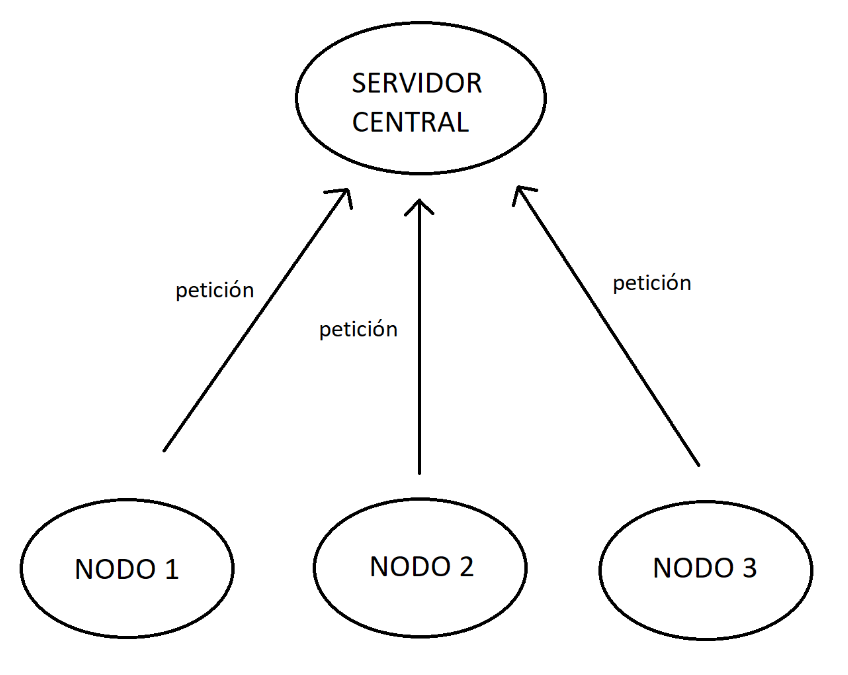
\includegraphics[width=0.5\textwidth]{images/exclusion_mutua.png}
    
\end{figure}
\subsection{Condición de carrera}
Una condición de carrera es un fenómeno que ocurre en sistemas concurrentes cuando el resultado de la ejecución depende del orden o la sincronización de eventos entre múltiples procesos o hilos. Sucede cuando el resultado de una operación depende del tiempo y la secuencia de ejecución de los procesos, y puede variar de una ejecución a otra. Las condiciones de carrera pueden surgir cuando varios procesos intentan acceder y modificar simultáneamente recursos compartidos sin la adecuada sincronización.
\begin{figure}[h]
    \centering
    \caption{Imagen que representa la Condición de carrera } 
    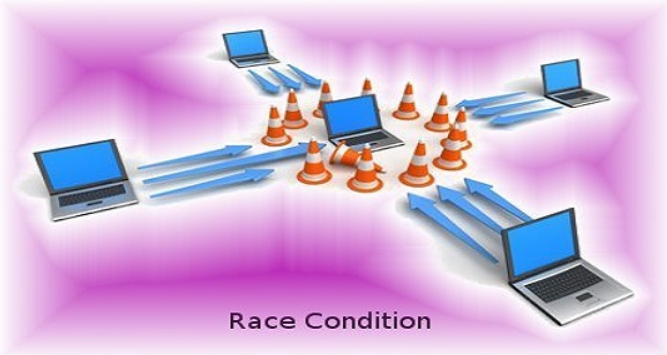
\includegraphics[width=0.5\textwidth]{images/condicion_carrera.png}
    
\end{figure}
\subsection{Deadlock}
Un deadlock, también conocido como \textbf{bloqueo mutuo}, es una situación en la que dos o más procesos o hilos quedan atrapados en un estado en el que ninguno puede continuar ejecutándose porque cada uno está esperando que el otro libere un recurso necesario. En otras palabras, los procesos se bloquean entre sí, creando un punto muerto en la ejecución del programa.
\espacio
Un deadlock generalmente ocurre cuando los procesos tienen acceso exclusivo a recursos compartidos y adquieren múltiples recursos pero los retienen mientras esperan la liberación de otros recursos que están en posesión de otros procesos.
\begin{figure}[h]
    \centering 
    \caption{Imagen que representa la Deadlock } 
    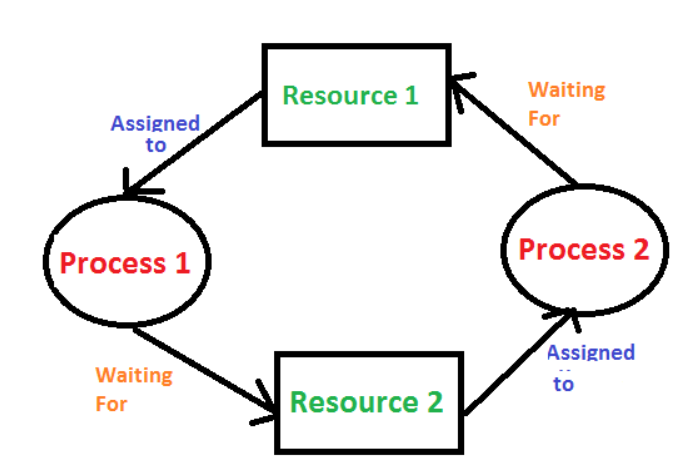
\includegraphics[width=0.5\textwidth]{images/Deadlock.png}
    
\end{figure}
\subsection{Starvation}
El \textbf{starvation} es un problema en sistemas concurrentes donde un proceso o hilo queda permanentemente excluido de acceder a un recurso o de completar su tarea, a pesar de que la planificación del sistema le permite ejecutarse. Este fenómeno ocurre cuando otros procesos o hilos en el sistema tienen prioridad sobre el proceso hambriento y monopolizan los recursos necesarios, impidiéndole avanzar.

\section{Problemas de Concurrencia}
\subsection{Inanición}
La \textbf{inanición} es un problema que ocurre en sistemas concurrentes cuando un proceso o hilo queda permanentemente excluido de acceder a recursos o de completar su tarea, a pesar de estar listo y esperando para ejecutarse. Este fenómeno se produce debido a que otros procesos en el sistema tienen prioridad sobre él y monopolizan los recursos necesarios, impidiéndole avanzar.

\subsection{Interbloqueo}
El interbloqueo, también conocido como \textbf{deadlock}, es una situación en la que dos o más procesos o hilos quedan atrapados en un estado en el que ninguno puede continuar ejecutándose porque cada uno está esperando que el otro libere un recurso necesario. En otras palabras, los procesos se bloquean entre sí, creando un punto muerto en la ejecución del programa.
\begin{figure}[htb!]
    \centering
    \caption{Imagen que representa la Interbloqueo } 
    \includegraphics[width=0.5\textwidth]{images/Interbloqueo.png}
    
\end{figure}
\subsection{Contención de recursos}
La contención de recursos se refiere a la competencia o disputa que surge cuando múltiples procesos o hilos intentan acceder a un recurso compartido al mismo tiempo. Esta situación puede conducir a conflictos y problemas de rendimiento si los recursos no están correctamente gestionados.

\section{Técnicas de sincronización}
\subsection{Monitores}
Los monitores son estructuras de control de acceso a recursos compartidos en programación concurrente. Fueron introducidos por C. A. R. Hoare en 1974 como una forma de sincronizar el acceso a datos compartidos entre múltiples procesos o hilos.
\espacio
Un monitor combina un tipo de datos abstracto (TDA) con un conjunto de procedimientos o métodos asociados, y proporciona un mecanismo de sincronización para garantizar que solo un hilo pueda ejecutar un procedimiento del monitor en un momento dado. Esto evita problemas de concurrencia, como las condiciones de carrera y los interbloqueos.\\
\subsubsection*{Los monitores constan de dos partes principales}
\begin{itemize}
    \item Variables y procedimientos internos: Estos son los datos y las operaciones que componen el TDA del monitor. Están protegidos por el monitor y solo pueden ser accedidos por los hilos a través de los procedimientos definidos en el monitor.
    \item Condición de espera y señalización: Los monitores incluyen un mecanismo para permitir que los hilos esperen a que se cumpla una determinada condición y luego sean notificados cuando esto sucede. Esto se logra mediante las operaciones de espera (wait) y señalización (signal) proporcionadas por el monitor.
    
\end{itemize}
\begin{figure}[htb!]
    \centering
    \caption{Imagen que representa las Monitores } 
    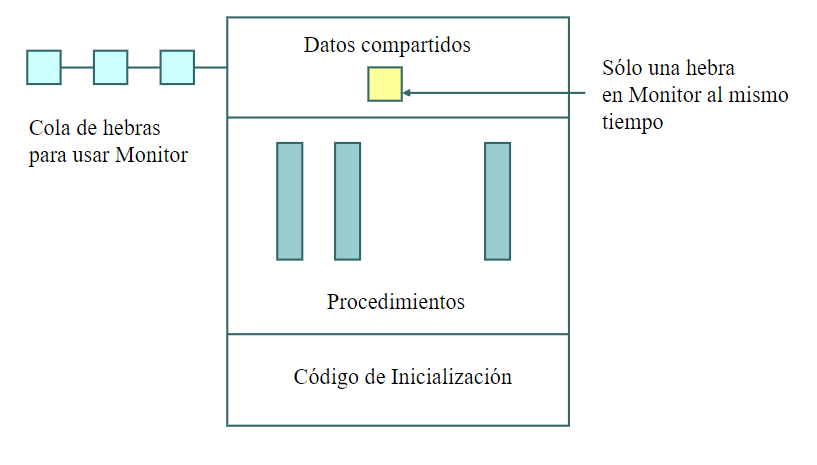
\includegraphics[width=0.5\textwidth]{images/monitor.png}
    
\end{figure}

\newpage
\subsection{Semáforos}
Los semáforos son una de las primitivas de sincronización más utilizadas en programación concurrente. Fueron propuestos por primera vez por Edsger Dijkstra en 1965 como un mecanismo para controlar el acceso a recursos compartidos entre procesos o hilos.
\espacio
Un semáforo es una variable entera que se utiliza para controlar el acceso a recursos compartidos mediante dos operaciones fundamentales:
\begin{itemize}
    \item P(s) (espera): Si el valor del semáforo es mayor que cero, se decrementa en uno y el proceso continúa su ejecución. Si el valor es cero, el proceso se bloquea hasta que el valor del semáforo sea mayor que cero.
    \item V(s) (señal): Incrementa el valor del semáforo en uno y despierta a uno de los procesos que estén esperando a que el valor del semáforo sea mayor que cero.
    
\end{itemize}
Los semáforos pueden tener diferentes variantes, como semáforos binarios (con valores 0 y 1), semáforos contadores (con valores no negativos) y semáforos mutex (para exclusión mutua).

\begin{figure}[htb!]
    \centering
    \caption{Imagen que representa los Semaforos } 
    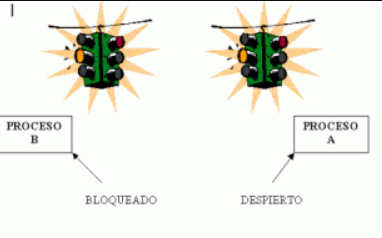
\includegraphics[width=0.5\textwidth]{images/semaforo.png}
    
\end{figure}
\subsection{Barreras}
Las barreras son estructuras de sincronización utilizadas en programación concurrente para coordinar la ejecución de múltiples hilos o procesos, asegurando que estos alcancen un punto de sincronización antes de continuar con la ejecución.
\espacio
Una barrera consta de un contador interno que se decrementa cada vez que un hilo o proceso alcanza la barrera. Cuando el contador alcanza cero, todos los hilos o procesos que esperan en la barrera pueden continuar con su ejecución.
\espacio
Las barreras son útiles cuando se necesita que todos los hilos o procesos lleguen a un punto de sincronización antes de proceder, como en el caso de dividir una tarea en subprocesos independientes que deben completarse antes de combinar los resultados.
\espacio
Las barreras son especialmente útiles en aplicaciones paralelas donde se realiza un procesamiento en paralelo y se necesita sincronizar los resultados parciales antes de continuar con la siguiente fase del procesamiento.
\section{Modelos de ejecución concurrente}
\subsection{Modelo de lectores-escritores}
El modelo de lectores-escritores es un problema clásico de sincronización en programación concurrente que involucra el acceso a un recurso compartido por múltiples procesos. En este modelo, hay dos tipos de procesos:

\begin{enumerate}
    \item \textbf{Lectores:} Procesos que solo leen el recurso compartido pero no lo modifican.
    \item \textbf{Escritores:} Procesos que leen y escriben en el recurso compartido.
     
\end{enumerate}
El objetivo del modelo es permitir el acceso concurrente de múltiples lectores al recurso compartido mientras se garantiza la exclusión mutua entre los escritores y entre un escritor y cualquier lector. Esto significa que los lectores pueden acceder al recurso compartido simultáneamente, pero los escritores deben tener un acceso exclusivo al recurso para evitar problemas de consistencia de datos.
\espacio
El modelo de lectores-escritores se puede implementar de varias maneras, utilizando diferentes técnicas de sincronización como semáforos, mutex, monitores u otras estructuras.

\subsubsection*{Algunas variantes del modelo incluyen:}
\begin{itemize}
    \item Lectores preferidos: Se da prioridad a los lectores sobre los escritores, lo que puede llevar a la inanición de los escritores si hay una alta concurrencia de lectores.
    \item Escritores preferidos: Se da prioridad a los escritores sobre los lectores, lo que puede llevar a la inanición de los lectores si hay una alta concurrencia de escritores.
    \item Alternancia justa: Se alterna entre lectores y escritores de manera justa para evitar la inanición de ambos.
    
\end{itemize}

\begin{figure}[htb!]
    \centering
    \caption{Imagen que representa el modelo Lector y Escritor  } 
    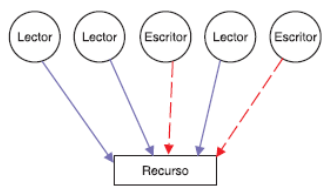
\includegraphics[width=0.5\textwidth]{images/lector.png}
    
\end{figure}


\subsection{Modelo de productor-consumidor}
El modelo de productor-consumidor es otro problema clásico de sincronización en programación concurrente, que involucra la coordinación entre dos tipos de procesos:
\begin{enumerate}
    \item \textbf{Productores:} Procesos que generan datos o recursos y los colocan en un búfer o cola compartida.
    \item \textbf{Consumidores:} Procesos que toman los datos o recursos del búfer o cola y los utilizan o procesan.
    
\end{enumerate}

El objetivo del modelo es permitir que los productores y consumidores trabajen de manera concurrente, evitando problemas como la sobreproducción o la falta de datos.
\cite{productor}
\espacio
El modelo de productor-consumidor se puede implementar utilizando una estructura de datos compartida, como un búfer o una cola, y mecanismos de sincronización, como semáforos o mutex, para garantizar la exclusión mutua y la sincronización entre los productores y consumidores.

\subsubsection*{Algunas variantes del modelo incluyen}
\begin{itemize}
    \item \textbf{Productor único, consumidor único:} Un único productor genera datos y un único consumidor los consume.
    \item \textbf{Productores múltiples, consumidor único:} Varios productores generan datos y un único consumidor los consume.
    \item \textbf{Productor único, consumidores múltiples:} Un único productor genera datos y varios consumidores los consumen.
    \item \textbf{Productores múltiples, consumidores múltiples:} Varios productores generan datos y varios consumidores los consumen.
    
\end{itemize}

\begin{figure}[htb!]
    \centering
    \caption{Imagen que representa el modelo Productor Consumidor } 
    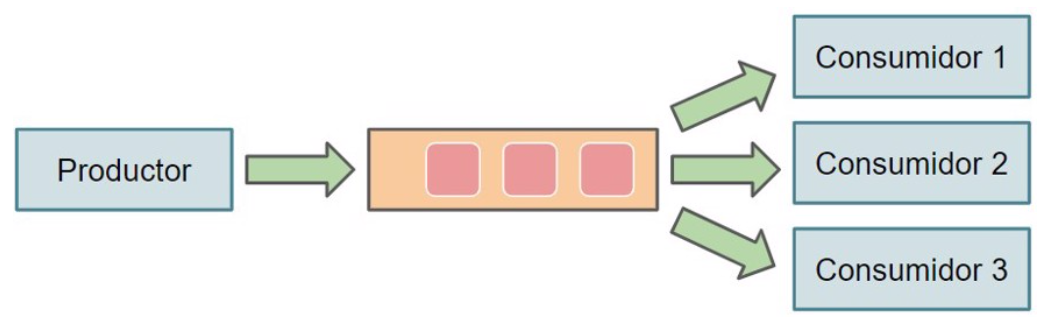
\includegraphics[width=0.5\textwidth]{images/productor.png}
    
\end{figure}
\subsection{Modelo de filósofos comensales}
El problema de los filósofos comensales, también conocido como el problema de los filósofos hambrientos, es un problema clásico de sincronización en programación concurrente propuesto por Edsger Dijkstra en 1965. Se plantea de la siguiente manera:
\cite{filosofo}
\espacio
Imagina que hay cinco filósofos sentados alrededor de una mesa redonda, y entre cada par de filósofos hay un tenedor. Cada filósofo pasa su tiempo pensando y comiendo. Para comer, un filósofo necesita usar los dos tenedores que están a su lado.
\espacio
El desafío consiste en diseñar un algoritmo de sincronización que permita a los filósofos alternar entre los estados de pensar y comer de manera segura, evitando posibles interbloqueos o inaniciones.

\subsubsection*{Algunas soluciones al problema de los filósofos comensales incluyen}

\begin{itemize}
    \item \textbf{Solución del camarero:} Introduce un camarero que controla el acceso a los tenedores y evita la competencia entre los filósofos por los recursos compartidos.
    \item \textbf{Solución de asignación de recursos:} Los filósofos adquieren los tenedores de uno en uno y los liberan en el mismo orden, evitando la posibilidad de interbloqueos.
    \item \textbf{Solución de jerarquía de recursos:} Se asigna un número a cada tenedor y se establece una jerarquía para su adquisición, evitando así ciclos de espera y garantizando que un filósofo pueda comer siempre y cuando pueda adquirir los tenedores de manera secuencial.
\end{itemize}

\begin{figure}[htb!]
    \centering
    \caption{Imagen que representa el modelo de los filosofos } 
    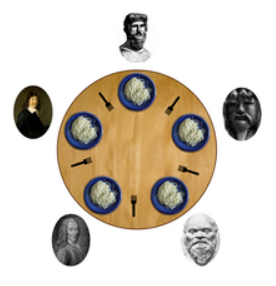
\includegraphics[width=0.5\textwidth]{images/filosofo.png}
    
\end{figure}


\newpage
\section{Referencias}
\bibliographystyle{apacite}
\bibliography{referencias.bib}


\end{document}